% Created by tikzDevice version 0.10.1 on 2017-12-04 15:15:28
% !TEX encoding = UTF-8 Unicode
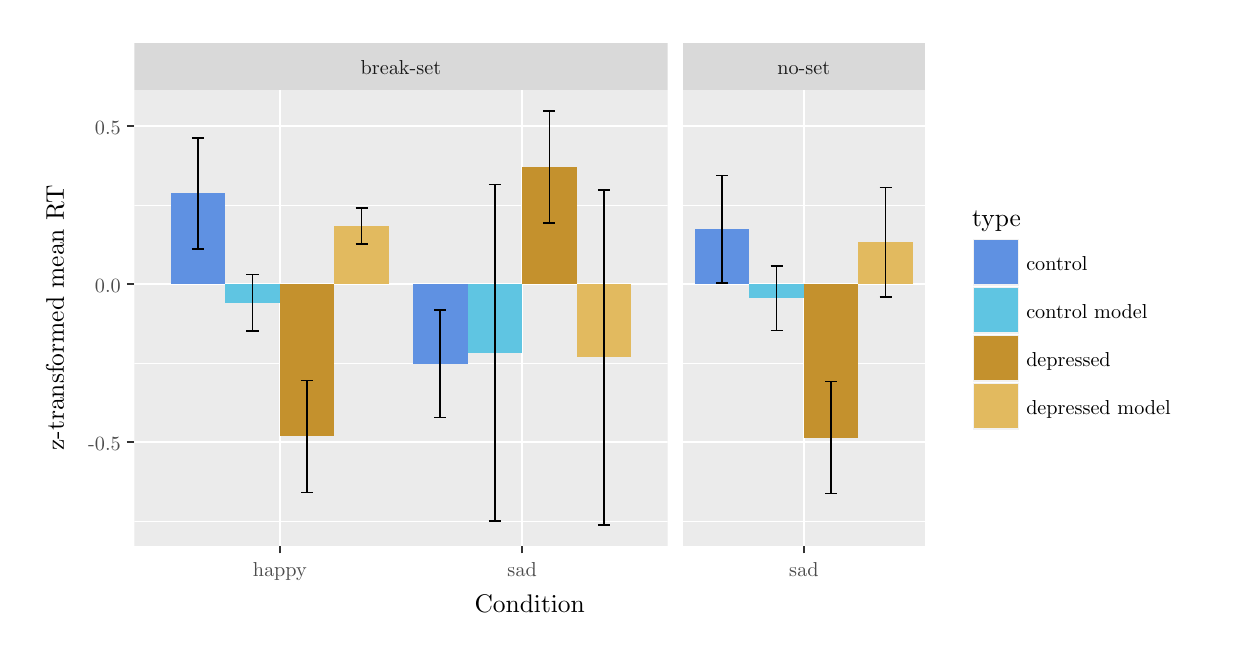
\begin{tikzpicture}[x=1pt,y=1pt]
\definecolor{fillColor}{RGB}{255,255,255}
\path[use as bounding box,fill=fillColor,fill opacity=0.00] (0,0) rectangle (433.62,216.81);
\begin{scope}
\path[clip] (  0.00,  0.00) rectangle (433.62,216.81);
\definecolor{drawColor}{RGB}{255,255,255}
\definecolor{fillColor}{RGB}{255,255,255}

\path[draw=drawColor,line width= 0.6pt,line join=round,line cap=round,fill=fillColor] ( -0.00,  0.00) rectangle (433.62,216.81);
\end{scope}
\begin{scope}
\path[clip] ( 38.57, 29.59) rectangle (231.20,194.25);
\definecolor{fillColor}{gray}{0.92}

\path[fill=fillColor] ( 38.57, 29.59) rectangle (231.20,194.25);
\definecolor{drawColor}{RGB}{255,255,255}

\path[draw=drawColor,line width= 0.3pt,line join=round] ( 38.57, 38.51) --
	(231.20, 38.51);

\path[draw=drawColor,line width= 0.3pt,line join=round] ( 38.57, 95.60) --
	(231.20, 95.60);

\path[draw=drawColor,line width= 0.3pt,line join=round] ( 38.57,152.68) --
	(231.20,152.68);

\path[draw=drawColor,line width= 0.6pt,line join=round] ( 38.57, 67.05) --
	(231.20, 67.05);

\path[draw=drawColor,line width= 0.6pt,line join=round] ( 38.57,124.14) --
	(231.20,124.14);

\path[draw=drawColor,line width= 0.6pt,line join=round] ( 38.57,181.23) --
	(231.20,181.23);

\path[draw=drawColor,line width= 0.6pt,line join=round] ( 91.11, 29.59) --
	( 91.11,194.25);

\path[draw=drawColor,line width= 0.6pt,line join=round] (178.66, 29.59) --
	(178.66,194.25);
\definecolor{fillColor}{RGB}{226,186,95}

\path[fill=fillColor] (110.81,124.14) rectangle (130.51,145.18);
\definecolor{fillColor}{RGB}{196,145,45}

\path[fill=fillColor] ( 91.11, 69.09) rectangle (110.81,124.14);
\definecolor{fillColor}{RGB}{95,197,226}

\path[fill=fillColor] ( 71.40,117.33) rectangle ( 91.11,124.14);
\definecolor{fillColor}{RGB}{95,145,226}

\path[fill=fillColor] ( 51.70,124.14) rectangle ( 71.40,156.91);
\definecolor{fillColor}{RGB}{226,186,95}

\path[fill=fillColor] (198.36, 97.64) rectangle (218.06,124.14);
\definecolor{fillColor}{RGB}{196,145,45}

\path[fill=fillColor] (178.66,124.14) rectangle (198.36,166.49);
\definecolor{fillColor}{RGB}{95,197,226}

\path[fill=fillColor] (158.96, 99.26) rectangle (178.66,124.14);
\definecolor{fillColor}{RGB}{95,145,226}

\path[fill=fillColor] (139.26, 95.39) rectangle (158.96,124.14);
\definecolor{drawColor}{RGB}{0,0,0}

\path[draw=drawColor,line width= 0.6pt,line join=round] (118.47,151.69) --
	(122.84,151.69);

\path[draw=drawColor,line width= 0.6pt,line join=round] (120.66,151.69) --
	(120.66,138.67);

\path[draw=drawColor,line width= 0.6pt,line join=round] (118.47,138.67) --
	(122.84,138.67);

\path[draw=drawColor,line width= 0.6pt,line join=round] ( 98.77, 89.36) --
	(103.14, 89.36);

\path[draw=drawColor,line width= 0.6pt,line join=round] (100.96, 89.36) --
	(100.96, 48.82);

\path[draw=drawColor,line width= 0.6pt,line join=round] ( 98.77, 48.82) --
	(103.14, 48.82);

\path[draw=drawColor,line width= 0.6pt,line join=round] ( 79.07,127.56) --
	( 83.44,127.56);

\path[draw=drawColor,line width= 0.6pt,line join=round] ( 81.26,127.56) --
	( 81.26,107.09);

\path[draw=drawColor,line width= 0.6pt,line join=round] ( 79.07,107.09) --
	( 83.44,107.09);

\path[draw=drawColor,line width= 0.6pt,line join=round] ( 59.37,176.92) --
	( 63.74,176.92);

\path[draw=drawColor,line width= 0.6pt,line join=round] ( 61.55,176.92) --
	( 61.55,136.90);

\path[draw=drawColor,line width= 0.6pt,line join=round] ( 59.37,136.90) --
	( 63.74,136.90);

\path[draw=drawColor,line width= 0.6pt,line join=round] (206.02,158.21) --
	(210.40,158.21);

\path[draw=drawColor,line width= 0.6pt,line join=round] (208.21,158.21) --
	(208.21, 37.07);

\path[draw=drawColor,line width= 0.6pt,line join=round] (206.02, 37.07) --
	(210.40, 37.07);

\path[draw=drawColor,line width= 0.6pt,line join=round] (186.32,186.76) --
	(190.70,186.76);

\path[draw=drawColor,line width= 0.6pt,line join=round] (188.51,186.76) --
	(188.51,146.23);

\path[draw=drawColor,line width= 0.6pt,line join=round] (186.32,146.23) --
	(190.70,146.23);

\path[draw=drawColor,line width= 0.6pt,line join=round] (166.62,160.09) --
	(171.00,160.09);

\path[draw=drawColor,line width= 0.6pt,line join=round] (168.81,160.09) --
	(168.81, 38.43);

\path[draw=drawColor,line width= 0.6pt,line join=round] (166.62, 38.43) --
	(171.00, 38.43);

\path[draw=drawColor,line width= 0.6pt,line join=round] (146.92,114.88) --
	(151.30,114.88);

\path[draw=drawColor,line width= 0.6pt,line join=round] (149.11,114.88) --
	(149.11, 75.89);

\path[draw=drawColor,line width= 0.6pt,line join=round] (146.92, 75.89) --
	(151.30, 75.89);
\end{scope}
\begin{scope}
\path[clip] (236.70, 29.59) rectangle (324.25,194.25);
\definecolor{fillColor}{gray}{0.92}

\path[fill=fillColor] (236.70, 29.59) rectangle (324.25,194.25);
\definecolor{drawColor}{RGB}{255,255,255}

\path[draw=drawColor,line width= 0.3pt,line join=round] (236.70, 38.51) --
	(324.25, 38.51);

\path[draw=drawColor,line width= 0.3pt,line join=round] (236.70, 95.60) --
	(324.25, 95.60);

\path[draw=drawColor,line width= 0.3pt,line join=round] (236.70,152.68) --
	(324.25,152.68);

\path[draw=drawColor,line width= 0.6pt,line join=round] (236.70, 67.05) --
	(324.25, 67.05);

\path[draw=drawColor,line width= 0.6pt,line join=round] (236.70,124.14) --
	(324.25,124.14);

\path[draw=drawColor,line width= 0.6pt,line join=round] (236.70,181.23) --
	(324.25,181.23);

\path[draw=drawColor,line width= 0.6pt,line join=round] (280.47, 29.59) --
	(280.47,194.25);
\definecolor{fillColor}{RGB}{226,186,95}

\path[fill=fillColor] (300.17,124.14) rectangle (319.88,139.30);
\definecolor{fillColor}{RGB}{196,145,45}

\path[fill=fillColor] (280.47, 68.69) rectangle (300.17,124.14);
\definecolor{fillColor}{RGB}{95,197,226}

\path[fill=fillColor] (260.77,119.06) rectangle (280.47,124.14);
\definecolor{fillColor}{RGB}{95,145,226}

\path[fill=fillColor] (241.07,124.14) rectangle (260.77,143.96);
\definecolor{drawColor}{RGB}{0,0,0}

\path[draw=drawColor,line width= 0.6pt,line join=round] (307.84,159.06) --
	(312.21,159.06);

\path[draw=drawColor,line width= 0.6pt,line join=round] (310.03,159.06) --
	(310.03,119.53);

\path[draw=drawColor,line width= 0.6pt,line join=round] (307.84,119.53) --
	(312.21,119.53);

\path[draw=drawColor,line width= 0.6pt,line join=round] (288.14, 88.90) --
	(292.51, 88.90);

\path[draw=drawColor,line width= 0.6pt,line join=round] (290.32, 88.90) --
	(290.32, 48.49);

\path[draw=drawColor,line width= 0.6pt,line join=round] (288.14, 48.49) --
	(292.51, 48.49);

\path[draw=drawColor,line width= 0.6pt,line join=round] (268.44,130.70) --
	(272.81,130.70);

\path[draw=drawColor,line width= 0.6pt,line join=round] (270.62,130.70) --
	(270.62,107.43);

\path[draw=drawColor,line width= 0.6pt,line join=round] (268.44,107.43) --
	(272.81,107.43);

\path[draw=drawColor,line width= 0.6pt,line join=round] (248.74,163.45) --
	(253.11,163.45);

\path[draw=drawColor,line width= 0.6pt,line join=round] (250.92,163.45) --
	(250.92,124.47);

\path[draw=drawColor,line width= 0.6pt,line join=round] (248.74,124.47) --
	(253.11,124.47);
\end{scope}
\begin{scope}
\path[clip] ( 38.57,194.25) rectangle (231.20,211.31);
\definecolor{fillColor}{gray}{0.85}

\path[fill=fillColor] ( 38.57,194.25) rectangle (231.20,211.31);
\definecolor{drawColor}{gray}{0.10}

\node[text=drawColor,anchor=base,inner sep=0pt, outer sep=0pt, scale=  0.73] at (134.88,199.75) {break-set};
\end{scope}
\begin{scope}
\path[clip] (236.70,194.25) rectangle (324.25,211.31);
\definecolor{fillColor}{gray}{0.85}

\path[fill=fillColor] (236.70,194.25) rectangle (324.25,211.31);
\definecolor{drawColor}{gray}{0.10}

\node[text=drawColor,anchor=base,inner sep=0pt, outer sep=0pt, scale=  0.73] at (280.47,199.75) {no-set};
\end{scope}
\begin{scope}
\path[clip] (  0.00,  0.00) rectangle (433.62,216.81);
\definecolor{drawColor}{gray}{0.20}

\path[draw=drawColor,line width= 0.6pt,line join=round] ( 91.11, 26.84) --
	( 91.11, 29.59);

\path[draw=drawColor,line width= 0.6pt,line join=round] (178.66, 26.84) --
	(178.66, 29.59);
\end{scope}
\begin{scope}
\path[clip] (  0.00,  0.00) rectangle (433.62,216.81);
\definecolor{drawColor}{gray}{0.30}

\node[text=drawColor,anchor=base,inner sep=0pt, outer sep=0pt, scale=  0.73] at ( 91.11, 18.58) {happy};

\node[text=drawColor,anchor=base,inner sep=0pt, outer sep=0pt, scale=  0.73] at (178.66, 18.58) {sad};
\end{scope}
\begin{scope}
\path[clip] (  0.00,  0.00) rectangle (433.62,216.81);
\definecolor{drawColor}{gray}{0.20}

\path[draw=drawColor,line width= 0.6pt,line join=round] (280.47, 26.84) --
	(280.47, 29.59);
\end{scope}
\begin{scope}
\path[clip] (  0.00,  0.00) rectangle (433.62,216.81);
\definecolor{drawColor}{gray}{0.30}

\node[text=drawColor,anchor=base,inner sep=0pt, outer sep=0pt, scale=  0.73] at (280.47, 18.58) {sad};
\end{scope}
\begin{scope}
\path[clip] (  0.00,  0.00) rectangle (433.62,216.81);
\definecolor{drawColor}{gray}{0.30}

\node[text=drawColor,anchor=base east,inner sep=0pt, outer sep=0pt, scale=  0.73] at ( 33.62, 64.02) {-0.5};

\node[text=drawColor,anchor=base east,inner sep=0pt, outer sep=0pt, scale=  0.73] at ( 33.62,121.11) {0.0};

\node[text=drawColor,anchor=base east,inner sep=0pt, outer sep=0pt, scale=  0.73] at ( 33.62,178.20) {0.5};
\end{scope}
\begin{scope}
\path[clip] (  0.00,  0.00) rectangle (433.62,216.81);
\definecolor{drawColor}{gray}{0.20}

\path[draw=drawColor,line width= 0.6pt,line join=round] ( 35.82, 67.05) --
	( 38.57, 67.05);

\path[draw=drawColor,line width= 0.6pt,line join=round] ( 35.82,124.14) --
	( 38.57,124.14);

\path[draw=drawColor,line width= 0.6pt,line join=round] ( 35.82,181.23) --
	( 38.57,181.23);
\end{scope}
\begin{scope}
\path[clip] (  0.00,  0.00) rectangle (433.62,216.81);
\definecolor{drawColor}{RGB}{0,0,0}

\node[text=drawColor,anchor=base,inner sep=0pt, outer sep=0pt, scale=  0.92] at (181.41,  5.50) {Condition};
\end{scope}
\begin{scope}
\path[clip] (  0.00,  0.00) rectangle (433.62,216.81);
\definecolor{drawColor}{RGB}{0,0,0}

\node[text=drawColor,rotate= 90.00,anchor=base,inner sep=0pt, outer sep=0pt, scale=  0.92] at ( 13.08,111.92) {z-transformed mean RT};
\end{scope}
\begin{scope}
\path[clip] (  0.00,  0.00) rectangle (433.62,216.81);
\definecolor{fillColor}{RGB}{255,255,255}

\path[fill=fillColor] (335.63, 65.58) rectangle (428.12,158.25);
\end{scope}
\begin{scope}
\path[clip] (  0.00,  0.00) rectangle (433.62,216.81);
\definecolor{drawColor}{RGB}{0,0,0}

\node[text=drawColor,anchor=base west,inner sep=0pt, outer sep=0pt, scale=  0.92] at (341.32,144.99) {type};
\end{scope}
\begin{scope}
\path[clip] (  0.00,  0.00) rectangle (433.62,216.81);
\definecolor{drawColor}{RGB}{255,255,255}
\definecolor{fillColor}{gray}{0.95}

\path[draw=drawColor,line width= 0.6pt,line join=round,line cap=round,fill=fillColor] (341.32,123.31) rectangle (358.67,140.65);
\end{scope}
\begin{scope}
\path[clip] (  0.00,  0.00) rectangle (433.62,216.81);
\definecolor{fillColor}{RGB}{95,145,226}

\path[fill=fillColor] (342.04,124.02) rectangle (357.96,139.94);
\end{scope}
\begin{scope}
\path[clip] (  0.00,  0.00) rectangle (433.62,216.81);
\definecolor{drawColor}{RGB}{255,255,255}
\definecolor{fillColor}{gray}{0.95}

\path[draw=drawColor,line width= 0.6pt,line join=round,line cap=round,fill=fillColor] (341.32,105.96) rectangle (358.67,123.31);
\end{scope}
\begin{scope}
\path[clip] (  0.00,  0.00) rectangle (433.62,216.81);
\definecolor{fillColor}{RGB}{95,197,226}

\path[fill=fillColor] (342.04,106.67) rectangle (357.96,122.60);
\end{scope}
\begin{scope}
\path[clip] (  0.00,  0.00) rectangle (433.62,216.81);
\definecolor{drawColor}{RGB}{255,255,255}
\definecolor{fillColor}{gray}{0.95}

\path[draw=drawColor,line width= 0.6pt,line join=round,line cap=round,fill=fillColor] (341.32, 88.62) rectangle (358.67,105.96);
\end{scope}
\begin{scope}
\path[clip] (  0.00,  0.00) rectangle (433.62,216.81);
\definecolor{fillColor}{RGB}{196,145,45}

\path[fill=fillColor] (342.04, 89.33) rectangle (357.96,105.25);
\end{scope}
\begin{scope}
\path[clip] (  0.00,  0.00) rectangle (433.62,216.81);
\definecolor{drawColor}{RGB}{255,255,255}
\definecolor{fillColor}{gray}{0.95}

\path[draw=drawColor,line width= 0.6pt,line join=round,line cap=round,fill=fillColor] (341.32, 71.27) rectangle (358.67, 88.62);
\end{scope}
\begin{scope}
\path[clip] (  0.00,  0.00) rectangle (433.62,216.81);
\definecolor{fillColor}{RGB}{226,186,95}

\path[fill=fillColor] (342.04, 71.98) rectangle (357.96, 87.91);
\end{scope}
\begin{scope}
\path[clip] (  0.00,  0.00) rectangle (433.62,216.81);
\definecolor{drawColor}{RGB}{0,0,0}

\node[text=drawColor,anchor=base west,inner sep=0pt, outer sep=0pt, scale=  0.73] at (360.84,128.95) {control};
\end{scope}
\begin{scope}
\path[clip] (  0.00,  0.00) rectangle (433.62,216.81);
\definecolor{drawColor}{RGB}{0,0,0}

\node[text=drawColor,anchor=base west,inner sep=0pt, outer sep=0pt, scale=  0.73] at (360.84,111.60) {control model};
\end{scope}
\begin{scope}
\path[clip] (  0.00,  0.00) rectangle (433.62,216.81);
\definecolor{drawColor}{RGB}{0,0,0}

\node[text=drawColor,anchor=base west,inner sep=0pt, outer sep=0pt, scale=  0.73] at (360.84, 94.26) {depressed};
\end{scope}
\begin{scope}
\path[clip] (  0.00,  0.00) rectangle (433.62,216.81);
\definecolor{drawColor}{RGB}{0,0,0}

\node[text=drawColor,anchor=base west,inner sep=0pt, outer sep=0pt, scale=  0.73] at (360.84, 76.91) {depressed model};
\end{scope}
\end{tikzpicture}
